\section{Experimental Evaluation}

In order to evaluate our approach and implementation, we applied
nondeterminism detection to three real world examples.  The primary
points we wanted to explore were (1) whether our approach was able to reliably detect actual
nondeterminism, (2) whether the overhead of nondeterminism
detection for real systems was acceptable, and (3) the performance of
delta-debugging for real nondeterministic predicates.

\subsection {Case Study: {\tt redis-py}}


\begin{figure*}
\centering 
\begin{subfigure}{0.67\columnwidth}
\centering
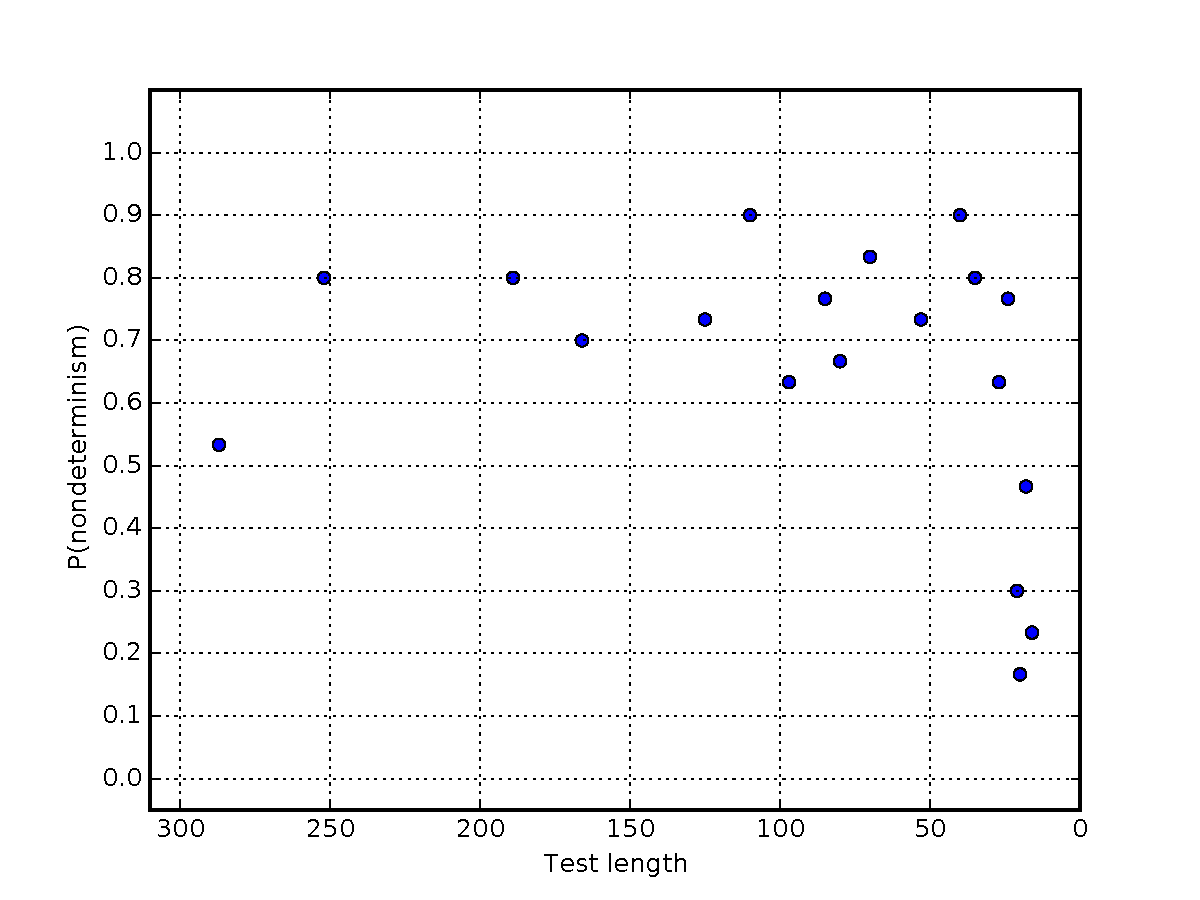
\includegraphics[width=\columnwidth]{redisddmin}
\caption{Standard delta-debugging (38s)}
\label{fig:r1}
\end{subfigure}
\begin{subfigure}{0.67\columnwidth}
\centering
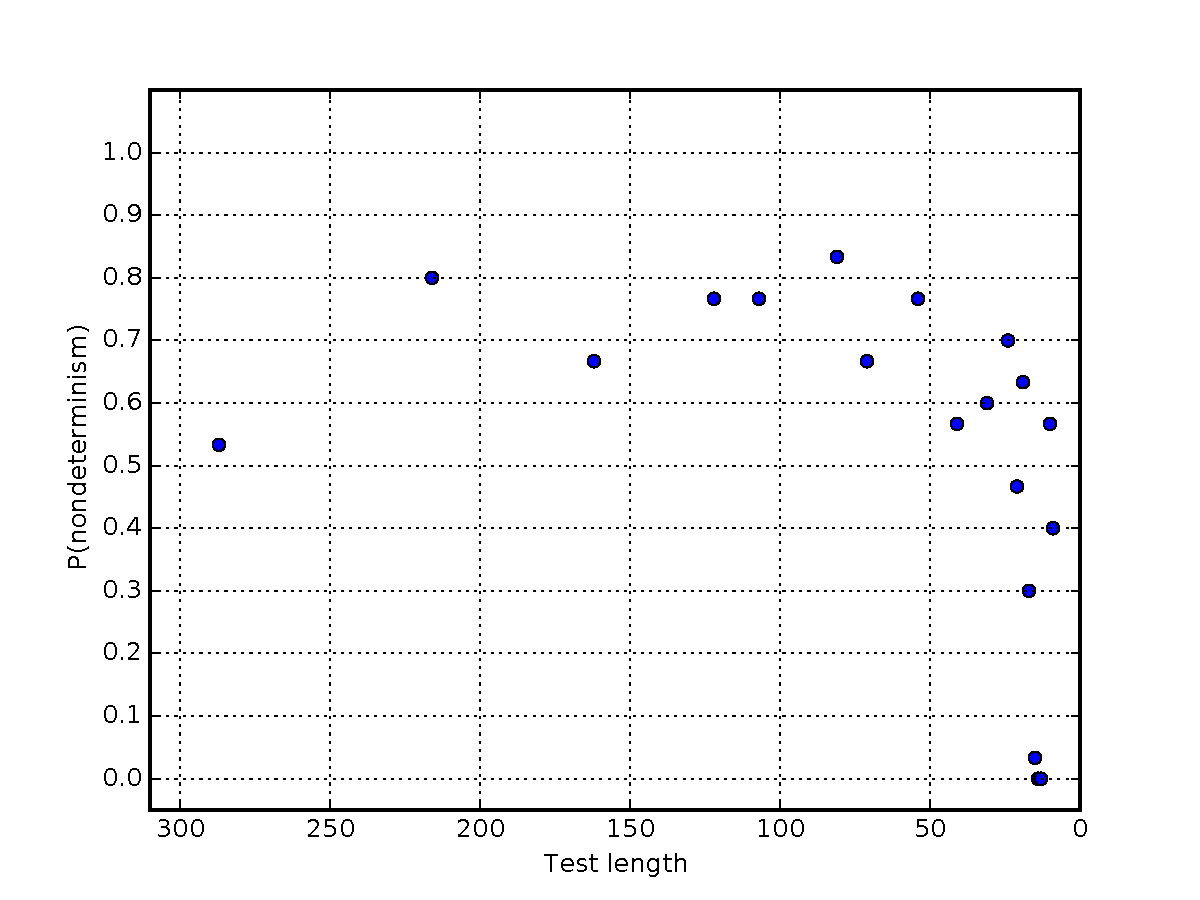
\includegraphics[width=\columnwidth]{redisforcep}
\caption{P=0.5, 100 samples (2131s)}
\label{fig:r2}
\end{subfigure}
\begin{subfigure}{0.67\columnwidth}
\centering
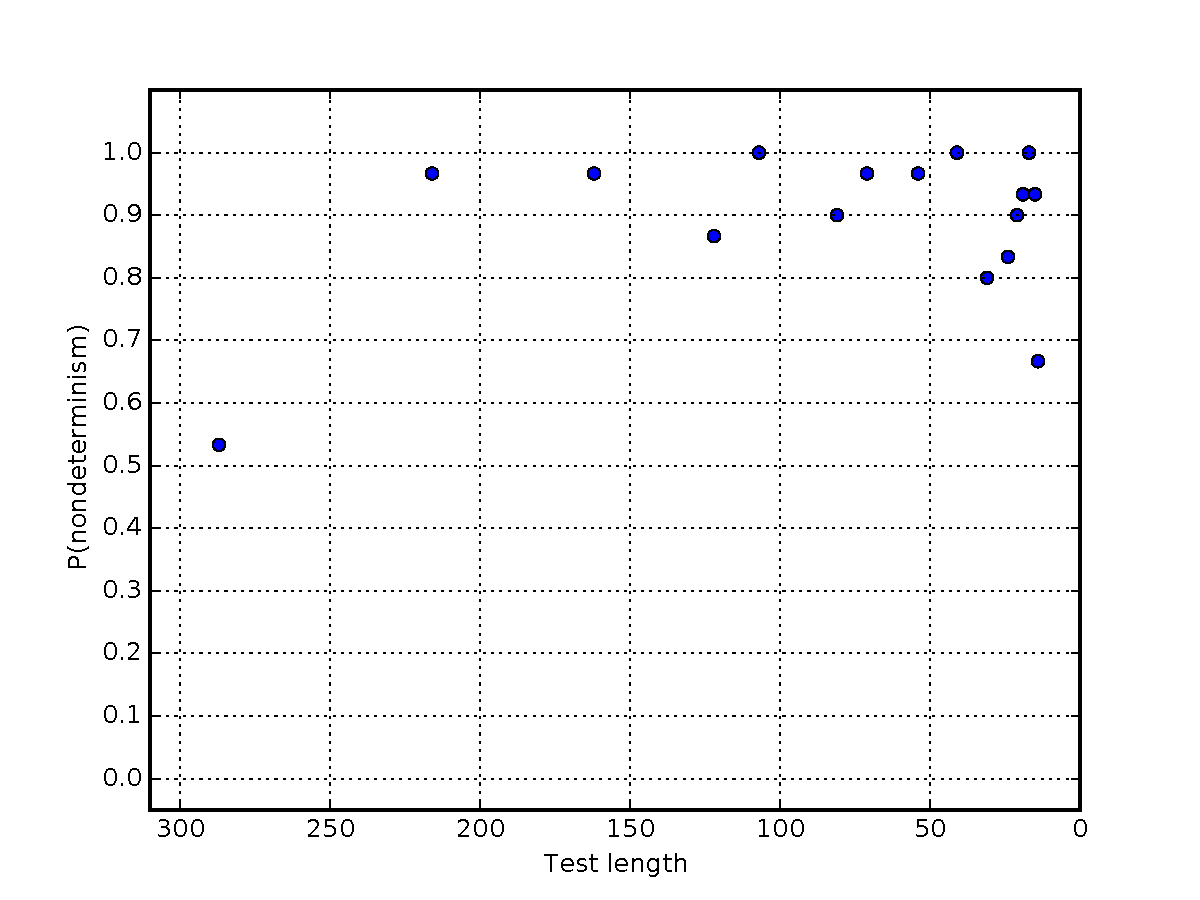
\includegraphics[width=\columnwidth]{redisforceprep}
\caption{P=0.5, 10 samples, 10 replications (617s)}
\label{fig:r3}
\end{subfigure}
\caption{Delta-debugging of the same {\tt redis-py} nondeterministic test}
\end{figure*}

The {\tt redis-py} \cite{redispy} module implements a widely-used Python interface
to the popular Redis in-memory database, cache, and
message broker \cite{redis}.

Using TSTL's harness for {\tt redis-py}, both {\tt redis-py} and Redis
itself can be tested; unfortunately, generating stand-alone
high-coverage regression tests for {\tt redis-py} and Redis using TSTL
has proven difficult, as numerous Redis commands introduce nondeterministic
behavior:  thus the resulting tests are very often \emph{flaky}.   Using {\tt tstl\_afl\_fuzz}, we can see that the {\tt redis-py} has a 
stability of only 56.26\%, a clear indicator of nondeterminism. Some
of the problematic commands are obvious simply by inspection (e.g.,
{\tt randomkey, srandmember}).  And, given an understanding of Redis
semantics, it is also clear that the various
commands producing data with a limited lifetime (e.g., {\tt expire,
  pexpire}) also introduce timing-based nondeterminism.


However, that a command such as {\tt restore} takes an expiration
argument is not obvious to a non-expert, nor is the behavior of {\tt
  spop} which pops a random value from a set.  Moreover, it is
difficult to guess whether the {\tt pipe} mechanism, which allows a
large sequence of commands to be queued up in a pipe and executed all
at once, introduced the potential for nondeterminism (does it execute
sequentially before other command are handled, or is it in parallel
with further commands).  Deep experience with Redis would make these
issues clear, but tests using a library are often written by those not
intimately familiar with the semantics of every used library (otherwise they would not have
been as likely to introduce flaky tests in the first place).  This is
even more true in the case of automated test generation, where the
test engineer is often chosen for expertise in test generation tools,
not in the domain of the software under test (SUT), and is seldom the
original developer of the code.

Using the original TSTL harness, just over 20\% of all {\tt redis-py}
regression tests (of length 200) generated were flaky.  Using the
nondeterminism checker to reduce flaky tests to a minimal set allows
us to simply set up an overnight run that will, in 12 hours, produce
a set of minimal flaky tests exposing the sources of
nondeterminism/flakiness.  In this case, the probability of flakiness
is not important, just the possibility, so we let the delta-debugging
create a minimal test with some non-zero (but possibly very small)
observed probability of nondeterminism.  

Figures \ref{fig:r1}-\ref{fig:r3} show delta-debugging of a typical
{\tt redis-py} nondeterministic test, originally with 287 steps.  The initial test behave
nondeterministically about half the time.  Figure \ref{fig:r1} shows
that this is a non-monotonic reduction problem, where removing steps
can either increase or decrease the probability of nondeterminism.  At
first, unmodified delta-debugging actually improves the probability of
failure, but eventually it produces a test of length 16 that only behaves
nondeterministically 24\% of the time.  The reduction takes only 38
seconds.  For the purpose of identifying commands leading to
nondeterminism, this is acceptable.  However, if we were actually
debugging a complex nondeterminism bug in Redis itself, we might want
a more reliably nondeterministic test.  Using the same parameters as
in Section \ref{sec:pubbias}, we see the same pattern.  Simply making
a predicate that ``forces'' the probability to remain high, with a
large number of samples, does not work (Figure \ref{fig:r3}) and
requires over 2000 seconds to produce a test with an even worse
probability of nondeterminism.  Using 10 samples and 10 replications,
on the other hand, actually improves the probability of
nondeterministic behavior, and
(in this case) even produces a smaller test (only 14 steps) in just
over 10 minutes.

After removing all identified sources of nondeterminism (the {\tt random-} functions, all
expiration-related functionality and {\tt restore} calls with non-zero
lifetimes, and {\tt spop}), but leaving all other suspect functionality in
place (e.g. pipes), no flakiness was observed in a sample of over 2,000 length
200 tests.  Moreover, because the removals were limited to actually
observed sources of flakiness, the code coverage loss was minimal.
Mean branch coverage, for regression tests of length 200 was reduced
by less than 5 branches (a less than 1\% decrease).  Obviously, it is
impossible to test the removed calls, but the overall coverage loss is
both minimal and known, and can be made up for using specially-crafted
tests (for instance, wrapping the problematic calls in a way that does
not check the values, or adding a delay after an expiration to allow
the data to expire).  As a price to pay for the ability to produce
fast-executing high-coverage full regression tests (not just tests for
crashes and unexpected exceptions), this seems acceptable.

Moreover, turning off sources of expected nondeterminism makes
it possible to aggressively test {\tt redis-py} and Redis for
unexpected nondeterminism arising from actual bugs.  The overhead for such
determinism checks, with no delay between operations, is only
20\%, much lower than the expected cost of running each test twice.
This is because choosing the actions in a test (and determining which
actions are enabled at each step) consumes a large part of the test
generator's time; running the test again and checking equality is
relatively inexpensive.  

Finally, AFL stability was 94.32\% with the harness allowing
nondeterminism, but rose to 98.32\% using the harness with
nondeterministic operations removed.

\subsection{Case Study: {\tt datarray} Inference Algorithms}

The {\tt datarray} module \cite{datarray} is a prototype
implementation for numpy arrays with named axes to improve data
management, developed by the Berkeley Institute for Data Science.  As part of its code, it provides a set of algorithms for
inference in
Bayesian belief networks \cite{russell2016artificial}.  An earlier
version of these algorithms produced nondeterministic (and in some
cases incorrect) results due to dependence on the order of values in
an iterator over a Python dictionary, on Python versions above 3.2, until 3.6 (see Section \ref{sec:pnondet}).

Figure \ref{hashbug} shows TSTL code for generating inputs to the {\tt
  datarray} algorithms.  The {\tt flatten\_and\_sort} function is needed because we care about actual differences in probability values, not simply the order of list, tuple, or dictionary items.  Running this harness using TSTL's {\tt
  --checkProcessDeterminism} flag required less than 10 seconds on
average to produce a test exhibiting process-level nondeterminism in
the {\tt calc\_marginals\_sumproduct} function (the only broken
algorithm).  Reducing this 60 step test to a minimal test of only 6 steps,
showing an extremely simple input producing the issue, 
required another 92 seconds.  Interestingly, the way that {\tt
  python-afl} is used in TSTL means that AFL stability is 100\%,
because the {\tt PYTHONHASHSEED} has already been chosen before the
fork in AFL executions.

Removing the nondeterministic call, we can see that the cost of
checking for process nondeterminism, with no delay between operations,
is high, a 93\% slowdown.  This is due to the high cost of subprocess
creation and communication.

\begin{figure*}
{\scriptsize
\begin{code}
@import inference\_algs
@import datarray
\vspace{0.1in}
<@
def flatten\_and\_sort(v):
    return (sorted(map(flatten\_and\_sort,v),key=repr) if type(v) in [list,tuple] else
                (flatten\_and\_sort(list(v.items())) if type(v) == dict else v))

def psplit(P):
    return ([P,1.0-P])
@>
\vspace{0.1in}
pool: <P> 3
pool: <cpts> 3
pool: <evidence> 3 OPAQUE
pool: <ename> 3
pool: <event> 3
\vspace{0.1in}
<P> := 0.01 * <[0..100]>
<ename> := "E" + str(<[1..5]>)
\{Exception\} <event> := datarray.DataArray(psplit(<P>), axes = [<ename>])
\{Exception\} <ename,1>!=<ename,2> -> <event> := [datarray.DataArray([[psplit(<P>)],psplit(<P>)],[<ename>,<ename>])]
<cpts> := []
~<cpts>.append(<event>)
<evidence> := \{\}
~<evidence>.update([(<ename>,0)])
\vspace{0.1in}
\{Exception\} print(flatten\_and\_sort(inference\_algs.calc\_marginals\_simple(<cpts>,<evidence>)))
\{Exception\} print(flatten\_and\_sort(inference\_algs.calc\_marginals\_sumproduct(<cpts>,<evidence>)))
\{Exception\} print(flatten\_and\_sort(inference\_algs.calc\_marginals\_jtree(<cpts>,<evidence>)))
\end{code}
}
\caption {Complete TSTL harness for finding the hash-order bug in the datarray
  inference algorithms.}
\label{hashbug}
\end{figure*}

\subsection {Vertical Determinism Case Study: {\tt pyfakefs}}

The {\tt pyfakefs} \cite{pyfakefs} module implements a fake file
system that mocks the Python file system modules, to allow Python
tests both to run faster by using an in-memory file system and to make
file system changes that would not be safe or easily performed using
real persistent storage.  Originally developed in 2006 at Google by
Mike Bland, {\tt pyfakefs} is now used in over 2,000 Python tests,
inside and outside Google \cite{pyfakefs}.

The TSTL harness for {\tt pyfakefs} has been used to detect (and
correct) over 80 faults.  However, the testing largely relies on
the existence of a reference file system implementation.  One purpose
of failure nondeterminism is to make it somewhat easier to perform
property-based testing of
complex APIs like this even without a reference implementation, or in cases
where the implementations do not use the same error
codes (as is common, e.g. in NASA flight software
\cite{ICSEDiff,CFV08}).

\subsubsection{Manually Inserted Fault}

We introduced a subtle bug into {\tt pyfakefs}, where the {\tt remove}
call checks that its target is not a directory, and returns the
correct error, but still carries out the remove operation.  Using {\tt
  os.remove} to delete directories does not break any file system
invariants, but violates the Python {\tt os} specification (and,
indirectly, the usual POSIX implementation behavior where {\tt unlink}
does not work for directories).  Detecting this bug using the TSTL
{\tt pyfakefs} harness is normally impossible without using another
file system as a reference.  However, the fault was detected
immediately, even without using a reference, when we compiled the harness
with the {\tt --checkFailureDeterminism} flag.  Because vertical
reduction does not require running complete tests multiple times, and
does not affect the delta-debugging algorithm's performance, reducing
the failing test to 3 steps required less than a second.
Moreover, the overhead for the check for failure determinism in a
version of the code without the {\tt remove} error was
less than 8\%.  Detecting the fault using a reference file system 
required 17\% more testing time before detection, and took over twice as
long to reduce the failure to a
slightly longer failing test, which did not have {\tt remove} as its
final operation (since further operations are required to 
expose the bad file system state the operation introduces).  For this
hypothetical subtle bug, failure determinism checks not only make it
possible to detect the fault without a reference implementation, it
improves on detection speed and ease of debugging even compared to a
full-blown reference implementation (the MacOS file system, operating
on a RAM disk) and strong, hand-tuned, differential testing.

\subsubsection{Mutation Analysis}

We wanted to determine whether there were also simple faults that
could be detected by failure nondeterminism, but \emph{not} detected
by differential testing, and quantify the additional specification
strength provided by failure determinism checks.  We therefore used
{\tt universalmutator} \cite{RegExpMut} to produce 2,350 mutants of
the {\tt pyfakefs} core file system code.   We restricted the generation
to only mutate code covered during a 60 second run of the test
harness, with differential testing turned off.  In this
\emph{non-differential} mode, the harness will only detect a fault when it
causes an unexpected exception to be raised, or results in a timeout
due to, e.g., an infinite loop.

We first analyzed the mutants using 60 seconds of non-differential
testing, then with the full differential test plus
an additional 60 seconds of testing (to make sure we accounted for the observed 17\%
extra time to detect in the manually constructed example: we want to
maximize the chance to detect a bug for the methods we compare
against).   For both comparisons, we then tested
the surviving mutants using the non-differential harness for 60
seconds, but with failure nondeterminism checking turned on.
We used the same random seed for
all runs, so that the only differences would be specification-based.

Non-differential testing, without failure determinism checks, killed
872 mutants, a 37.1\% kill rate.  Adding a failure determinism check
allowed the testing to kill an additional 98 mutants, an 11\% improvement.
The differential harness, with an additional 60 seconds of testing
time, killed 1148 mutants, improving the kill rate to 48.8\%.  Failure determinism added an
additional 71 mutants to the total killed, a 6\% improvement even for
this strong differential harness with a larger test budget.  The kill rates are generally low
because {\tt universalmutator}, by design, includes many operations
that can produce equivalent mutants, but can also produce hard-to-kill
non-equivalent mutants not produced by other mutation tools, e.g. code
that throws away exceptions raised by a function call, or code
reversing a list.

In order to further investigate the additional specification power
provided by failure nondeterminism detection, we inspected the mutants
killed using the failure determinism check but not killed by the
strong differential testing.  The largest category of mutants not
killed (22 of the 71 mutants) was what we refer to as ``exception
swallowing'' mutants, which transform a Python statement into the same
statement, but wrapped in a {\tt try} block with a catch that ignores
any raised exceptions, e.g., {\tt foo()} becomes:

\begin{code}
try: foo()
except: pass
\end{code}

\noindent It is easy to
see that such mutants may introduce faults in the handling of
errors, and thus would tend to cause failure nondeterminism.  However,
these are a minority of the mutations introducing hard-to-detect but
non-equivalent failure
nondeterminism.  Other mutation operators resulting in subtle flaws
not (at least easily) detectable by differential testing compared to a
correct file system include:  arithmetic operation changes, statement
deletions, logical operator modifications, constant replacements
(including replacement of a string with the empty string), and
introducing a break into a loop.  The variety of mutant types suggests
that no more specifically tailored strategy such as checking for
exception propagation, will work as well as introducing a notion of
failure nondeterminism.

We also checked the cost of introducing failure determinism checking
by analyzing mutants that could be killed by both methods.  Even
though in some cases the failure determinism check allows a mutant to
be detected sooner, the mean time to kill mutants was 0.006 seconds
larger with failure determinism checking, and this change was significant by Wilcoxon test
$(p < 1 \times 10^{-15})$.  While significant, this cost is probably
too small to be of any real practical importance.
